\documentclass[12pt, oneside]{extbook}

\usepackage[utf8]{inputenc}
\usepackage[T1]{fontenc}
\usepackage[italian]{babel}
\usepackage{tabularx}
\usepackage{wrapfig}
% Font simile a Times New Roman per testo e matematica
\usepackage{newtxtext,newtxmath}

% Pacchetti aggiuntivi necessari per il frontespizio
\usepackage{graphicx} % Per includere l'immagine
\usepackage{setspace} 

\usepackage{tikz}
\usetikzlibrary{shapes,arrows,positioning}
\usepackage{float}

% Impostazioni di formattazione pagina (Definizione Generale)
\usepackage{geometry}
\geometry{
  a4paper,
  top=3cm,
  bottom=4cm,
  left=3.5cm,% Margine sinistro (Ora fisso su tutte le pagine)
  right=3.5cm% Margine destro (Ora fisso su tutte le pagine)
}

% Interlinea doppia
\doublespacing
\setlength{\parindent}{0pt}

% ======================================================================
% INTESTAZIONE / PIÈ DI PAGINA: NUMERO CENTRATO IN BASSO
% ======================================================================
\usepackage{fancyhdr}
\pagestyle{fancy}
\fancyhf{}             % pulisce header e footer
\fancyfoot[C]{\thepage}    % numero di pagina centrato in basso
\renewcommand{\headrulewidth}{0pt} % niente linea in alto
\renewcommand{\footrulewidth}{0pt} % niente linea in basso

% ======================================================================
% --- MACRO: INFORMAZIONI DELLA TESI (da personalizzare) ---
% ======================================================================
\newcommand{\universita}{UNIVERSITÀ DEGLI STUDI DI SASSARI}
\newcommand{\dipartimento}{Dipartimento di Ingegneria}
\newcommand{\corso}{Corso di Laurea in Ingegneria Informatica}
\newcommand{\titolo}{Analisi Geospaziale delle Emissioni Inquinanti del Traffico Veicolare}
\newcommand{\relatore}{Dott. Ruiu Pietro}
\newcommand{\corelatore}{Dott. Lagorio Andrea}
\newcommand{\candidato}{Pinna Fabrizio}
\newcommand{\annoaccademico}{2024/2025}

% Macro per lo stemma (DIMENSIONE 7cm)
\newcommand{\logoimg}{
\includegraphics[width=7cm]{foto/logo_uniss_versione_base_orizzontale_sfondo_trasparente_0.png}}


\begin{document}

% ======================================================================
% FRONTESPIZIO (PRIMA PAGINA)
% ======================================================================
\begin{titlepage}

    % A. IMPOSTAZIONE MARGINI SIMMETRICI PER LA SOLA PRIMA PAGINA (per centrare perfettamente)
    \newgeometry{
        a4paper,
        top=2.5cm, 
        bottom=2.5cm,
        left=3.5cm, % Margini simmetrici temporanei per la centratura
        right=3.5cm,
        headheight=0pt, 
        foot=0pt 
    }
    
    \singlespacing % Disattiva l'interlinea doppia solo per il frontespizio

    \centering % Centra orizzontalmente tutto il contenuto della pagina

    % 1. PARTE SUPERIORE: STEMMA E UNIVERSITÀ (Compattato)
    \vspace*{0.3cm} % Spostato più in alto
    
    {\logoimg \par} % CHIAMA LA MACRO PER L'IMMAGINE
    
    \vspace{2cm} % Spazio ridotto
    
    {\Huge \bfseries \universita \par} % Università in grassetto e grande
    \vspace{0.6cm} % Spazio ridotto
    
    % 2. DIPARTIMENTO E CORSO DI LAUREA
    {\large \dipartimento \par}
    {\large \corso \par}
    \vspace{3.5cm} % Spazio ridotto prima del titolo

    % 3. TITOLO DELLA TESI
    \begin{minipage}{0.95\textwidth} % Larghezza 95%
        \centering
        \linespread{1.3}\selectfont 
        {\Huge \bfseries \titolo \par} % Titolo Molto Grande e Grassetto
    \end{minipage}
    \linespread{1.0}\selectfont % Ripristina spaziatura normale
    \vspace{2.5cm} % Spazio dopo il titolo

    \vfill % SPAZIO FLESSIBILE: SPINGE IL CONTENUTO SUCCESSIVO IN FONDO

    % 4. INFORMAZIONI RELATORI E CANDIDATO (Sinistra e Destra)
    \noindent % Fondamentale per allineare ai margini
    \begin{minipage}[t]{0.45\textwidth} % BLOCCO SINISTRO (Relatore/Co-Relatore)
        \raggedright 
        \textbf{Relatore:} \par
        \relatore \par
        \vspace{0.8cm}
        
        \textbf{Co-Relatore:} \par
        \corelatore \par
    \end{minipage}%
    \hfill% Spazio orizzontale massimo
    \begin{minipage}[t]{0.45\textwidth} % BLOCCO DESTRO (Candidato)
        \raggedleft % Allinea a destra
        \textbf{Tesi di laurea di:} \par
        \candidato \par
    \end{minipage}
    \par % Finisce la riga dei minipages
    
    \vspace{2.0cm} % Spazio per separare i blocchi dall'anno
    
    % 5. ANNO ACCADEMICO (Centrato)
    \centering
    {\large Anno Accademico \annoaccademico \par} % Anno accademico centrato
    
    \vspace{0.5cm} % Spazio finale
    
    % RIPRISTINO DEI MARGINI ORIGINALI PER LE PAGINE SUCCESSIVE
    \restoregeometry
    
\end{titlepage}

\newpage
\thispagestyle{empty}
\mbox{}
\newpage


\section*{Riconoscimenti}

Esprimo la mia profonda riconoscenza a tutti coloro che hanno contribuito alla realizzazione di questo progetto.

Un ringraziamento speciale va al relatore, Dott. Pietro Ruiu}, per la sua preziosa supervisione e per la chiarezza incisiva con cui ha aiutato a definire e centrare gli obiettivi fondamentali di questa tesi.

La mia gratitudine si estende in particolar modo al co-relatore, Dott. Andrea Lagorio, il cui supporto è stato cruciale nell'articolazione dell'intero percorso di sviluppo e per le indicazioni mirate fornite in ogni fase del processo.

Infine, ringrazio l'Università degli Studi di Sassari per le opportunità accademiche fornite che hanno permesso di completare questo lavoro.

\newpage
\thispagestyle{empty}
\mbox{}
\newpage


\tableofcontents

\newpage
\thispagestyle{empty}
\mbox{}
\newpage


% ======================================================================
% CAPITOLO 1 - INTRODUZIONE
% ======================================================================

\chapter{Introduzione}

\section{Contesto, Problema e Motivazione}
\label{sec:contesto}
L'inquinamento atmosferico rappresenta oggi una delle principali criticità ambientali e sanitarie nelle aree urbane.
Tra le diverse sorgenti emissive, il \textbf{traffico veicolare} è riconosciuto a livello internazionale come uno dei contributori più rilevanti alle concentrazioni di inquinanti nell'ambiente.

Il lavoro si fonda sull’idea che i soli conteggi di veicoli (auto, bus, moto, camion) non siano sufficienti a rappresentare in modo adeguato l’impatto del traffico sulla qualità dell’aria.
Negli ultimi anni, i \textbf{Conteggi di Transito Veicolare} sono diventati più facili da raccogliere grazie a sensori IoT e telecamere, ma spesso vengono forniti in forma grezza (ad esempio, file \texttt{TXT} o \texttt{CSV}) e poco strutturata, risultando quindi non immediatamente utilizzabili per analisi ambientali.

Il \textbf{problema} principale affrontato nella tesi è proprio questo divario: la necessità di trasformare un flusso grezzo di dati di traffico in una stima della massa di inquinante emesso.
Per compiere questa transizione è indispensabile integrare modelli di \textbf{Fattori di Emissione} (Emission Factors, EF) e introdurre assunzioni specifiche sul tratto di strada a cui i dati si riferiscono.
Nella pratica attuale, questi elementi cruciali vengono raramente gestiti insieme al dato grezzo e rimangono spesso dispersi tra documentazione tecnica, fogli di calcolo e codice.

Le motivazioni alla base dello sviluppo del lavoro sono essenzialmente due.
Da un lato, la necessità di disporre di una soluzione tecnica in grado di gestire grandi volumi di dati di traffico.
Dall’altro, l’esigenza di disporre di uno strumento di \textbf{visualizzazione dinamica} che consenta di tradurre i conteggi veicolari in informazioni ambientali facilmente leggibili anche da chi non ha una formazione specialistica in modellistica dell’inquinamento.

\section{Obiettivi del Progetto e Risultati Attesi}

L'obiettivo generale della tesi è la realizzazione di una piattaforma web interattiva e \emph{data-driven} che, a partire da dati di traffico ricavati da telecamere o sensori, fornisca una visualizzazione dell'impatto emissivo stimato sul territorio.

In termini più operativi, il lavoro può essere scomposto in alcuni obiettivi specifici, che si possono riassumere come segue.

\subsection{Sviluppo di un sistema completo per l'acquisizione, l'elaborazione e la visualizzazione dei dati di traffico}

Il primo obiettivo consiste nel definire un'architettura \emph{full-stack} (PHP/MySQL e JavaScript) che gestisca l'intero ciclo di vita del dato, dal caricamento alla visualizzazione sulla mappa.

In concreto sono stati realizzati:
\begin{itemize}
\item un'interfaccia di \textbf{upload} lato server che si occupa di leggere il file, validarlo e aggregare i dati in intervalli temporali (time bucketing);
\item un'API di \textbf{interrogazione} che restituisce i dati aggregati in base ai filtri richiesti dall'utente (intervallo temporale e area geografica).
\end{itemize}

\subsection{Implementazione di un modello dinamico per la stima delle emissioni}

Il secondo obiettivo riguarda l'integrazione dei \textbf{Fattori di Emissione} ($g/\text{veicolo} \cdot \text{km}$) nel modello dati e l'implementazione del relativo calcolo lato client.
Il sistema combina i conteggi veicolari con i fattori di emissione per tipo di veicolo (ad esempio auto, camion) e per inquinante (ad esempio $\text{PM}{10}$, $\text{NO}{\text{X}}$), restituendo la massa di inquinante stimata per ciascun punto osservato.

\subsection{Creazione di un'interfaccia web per l'analisi dei dati storici e in tempo reale}

Il terzo obiettivo è la realizzazione di un'interfaccia web basata su \textbf{Leaflet} e \textbf{Circle Marker} per rappresentare sulla mappa, in modo dinamico, sia il conteggio veicolare sia l'emissione stimata.
La scala cromatica e le dimensioni dei marker (stile heatmap) sono definite da una logica di stilizzazione dedicata.

L'utente può scegliere:
\begin{itemize}
\item la \textbf{metrica} da visualizzare (conteggio grezzo o emissione);
\item la \textbf{categoria veicolare} (ad esempio solo veicoli pesanti oppure il totale);
\item l'intervallo \textbf{temporale} (singolo giorno o intervallo di date).
\end{itemize}

La piattaforma include inoltre strumenti di supporto, come grafici a torta e un \emph{player} giornaliero, che permettono di esplorare nel dettaglio l'andamento giornaliero del traffico e delle emissioni.

% ======================================================================
% CAPITOLO 2 - I DATI DI INGRESSO E LA LORO ACQUISIZIONE
% ======================================================================

\chapter{I Dati di Ingresso e la Loro Acquisizione}

Il punto di partenza di ogni analisi è la qualità e la struttura dei dati grezzi. In questo capitolo vengono descritti la natura dei conteggi veicolari utilizzati, il processo che li genera e il formato con cui vengono forniti al sistema.

\section{Telecamere di Monitoraggio e Dati Rilevati}

I dati grezzi analizzati derivano da un processo di \emph{video detection} basato su rete neurale (modello YOLO) e \emph{tracking} degli oggetti. Ogni telecamera, installata nel comune di \textbf{Portici (NA)}, inquadra un incrocio o un tratto di strada critico e produce, tramite questo sistema, una sequenza di frame annotati. Le Figure~\ref{fig:via-liberta} e~\ref{fig:via-diaz-moro} mostrano due
esempi di inquadrature reali utilizzate nel progetto. In entrambe le
scene sono visibili i \emph{bounding box} generati dal modello di
rilevamento per ciascun veicolo, insieme al relativo identificativo di tracking.

\begin{figure}[H]
  \centering
  \vspace{-0.3cm}
  \includegraphics[width=0.95\textwidth]{foto/via_liberta_via_verdi.png}
  \caption{Telecamera di \emph{Via Libertà / Via Verdi}. I veicoli sono evidenziati da rettangoli con etichetta della classe e identificativo di tracking.}
  \label{fig:via-liberta}
  \vspace{-0.2cm}
\end{figure}

\begin{figure}[H]
  \centering
  \vspace{-0.5cm}
  \includegraphics[width=0.95\textwidth]{foto/via_diaz_moro.png}
  \caption{Telecamera di \emph{Via Diaz--Moro}. Ogni veicolo è tracciato tramite \emph{bounding box} e \texttt{track\_id} univoco.}
  \label{fig:via-diaz-moro}
  \vspace{-0.5cm}
\end{figure}

\newpage

Ogni telecamera produce quindi, tramite il sistema di detection e tracking, una sequenza di frame annotati. Di ciascun veicolo non viene
memorizzata l’immagine, ma soltanto i metadati essenziali necessari al
conteggio: il frame in cui compare e la durata complessiva della
traccia, la categoria veicolare (auto, moto, bus, camion), la posizione
del veicolo nell’immagine (centro e dimensioni del \emph{bounding box})
e l’identificativo univoco \texttt{track\_id}. 

A partire da questi
metadati è possibile ricostruire i passaggi di veicoli nell’arco del
tempo e convertirli in conteggi aggregati per intervallo temporale e per
categoria.

\begin{figure}[H]
\centering
\begin{tikzpicture}[
  node distance=0.5cm,
  block/.style={
    rectangle,
    rounded corners=3pt,
    draw=black,
    thick,
    text width=2.2cm,
    minimum height=0.9cm,
    font=\scriptsize,
    align=center
  },
  flow/.style={->, thick, >=latex}
]

\node[block, fill=blue!15] (video) {Video\\telecamera};
\node[block, fill=green!15, right=0.5cm of video] (yolo) {Rilevamento e\\tracking (YOLO)};
\node[block, fill=yellow!20, right=0.5cm of yolo] (txt) {File\\TXT/CSV};
\node[block, fill=orange!20, right=0.5cm of txt] (agg) {Aggregazione\\a intervalli};
\node[block, fill=red!20, right=0.5cm of agg] (count) {Conteggi\\veicolari\\aggregati};

\draw[flow] (video) -- (yolo);
\draw[flow] (yolo) -- (txt);
\draw[flow] (txt) -- (agg);
\draw[flow] (agg) -- (count);

\end{tikzpicture}

\caption{Flusso di estrazione dei dati dal video: dalla rilevazione dei veicoli alla generazione dei conteggi aggregati.}
\label{fig:flusso-video}
\end{figure}




\section{Formato del File di Input}

Per ogni telecamera viene generato un file di testo, in formato \texttt{TXT}, che contiene una riga per ogni
veicolo rilevato in ogni frame del video. La struttura logica del file è la
seguente:

\begin{verbatim}
<frame rate>

<frame> <classe> <cx> <cy> <w> <h> <track_id>
\end{verbatim}

Il valore iniziale \texttt{frame rate} rappresenta il numero di frame al
secondo del video analizzato e viene utilizzato per convertire i numeri
di frame in tempo reale. Per ogni riga successiva, il campo
\texttt{frame} indica il numero progressivo del frame in cui il
veicolo è stato rilevato, mentre \texttt{classe} è l’ID numerico della
classe di oggetto riconosciuta (nel caso specifico: 2 per le auto,
3 per le motociclette, 5 per i bus e 7 per i camion). I valori
\texttt{cx} e \texttt{cy} rappresentano le coordinate normalizzate del
centro del \emph{bounding box}, comprese tra 0 e 1 rispetto a larghezza
e altezza dell’immagine; \texttt{w} e \texttt{h} sono invece la
larghezza e l’altezza normalizzate del riquadro. 

Infine,
\texttt{track\_id} è l’identificativo univoco assegnato dal modulo di
tracking al singolo veicolo e consente di seguire lo stesso oggetto su
più frame consecutivi. Queste informazioni costituiscono la base per il successivo conteggio dei passaggi e per l’aggregazione in intervalli temporali regolari, che rappresentano l’input principale delle fasi di calcolo delle emissioni e di visualizzazione sulla mappa.

\begin{figure}[H]
  \centering
  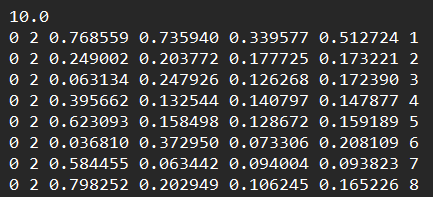
\includegraphics[width=0.95\textwidth]{foto/Immagine 2025-11-19 132757.png}
  \caption{Estratto file yolo.txt}
  \vspace{-0.5cm}
\end{figure}



% ======================================================================
% CAPITOLO 3 - FONDAMENTI TEORICI
% ======================================================================

\chapter{Fondamenti Teorici e Modelli di Riferimento}

In questo capitolo si introducono i concetti teorici alla base della piattaforma:
gli inquinanti considerati, i Fattori di Emissione e il modello matematico
utilizzato per stimare le emissioni a partire dai conteggi veicolari. Si richiamano
anche alcuni principi generali legati alla rappresentazione geospaziale dei
dati.

\section{L'Inquinamento da Sorgenti Mobili e Fattori di Emissione (EF)}

Il traffico veicolare è una sorgente importante di inquinamento atmosferico e
produce numerose sostanze nocive. In questa tesi ci si concentra in particolare su:

\begin{itemize}
  \item \textbf{Ossidi di Azoto ($\text{NO}_{\text{X}}$):} gas che contribuiscono
        alla formazione di smog fotochimico e piogge acide.
  \item \textbf{Particolato (PM$_{10}$ e $\text{PM}_{2.5}$):} particelle solide
        o liquide di piccole dimensioni, generate sia dallo scarico
        (particolato primario) sia dall'usura di freni, pneumatici e manto
        stradale (particolato secondario).
  \item \textbf{Monossido di Carbonio ($\text{CO}$):} gas incolore e inodore
        prodotto dalla combustione incompleta, particolarmente rilevante nei
        contesti urbani con forte traffico.
\end{itemize}

Per passare dal traffico veicolare alle emissioni si utilizza il concetto di
\textbf{Fattore di Emissione (EF)}. Il Fattore di Emissione è un coefficiente
che esprime la massa di inquinante emessa per unità di attività. Nel caso dei
veicoli, l'unità di attività è in genere il \emph{veicolo-chilometro}, e il
fattore viene quindi espresso in grammi per veicolo-chilometro
($g/\text{veicolo}\cdot\text{km}$).

\subsection{Fonte dei Fattori di Emissione: ISPRA}

I Fattori di Emissione utilizzati in questa tesi derivano dalle banche dati ufficiali fornite da \textbf{ISPRA} (Istituto Superiore per la Protezione e la Ricerca Ambientale). ISPRA è l'ente tecnico-scientifico di riferimento a livello nazionale per le tematiche ambientali e produce, tra le altre cose, l'inventario nazionale delle emissioni in atmosfera. 

I valori specifici utilizzati in questa analisi sono stati calcolati utilizzando il software \textbf{COPERT} (versione 5.7.3), il cui sviluppo è coordinato dall'Agenzia Europea dell'Ambiente. Le metodologie adottate sono coerenti con gli standard europei (\emph{EMEP/EEA air pollutant emission inventory guidebook 2023}) e con le \emph{Guidelines IPCC 2006}. I dati sono pubblicamente consultabili attraverso la banca dati ufficiale, accessibile al seguente indirizzo: \url{https://fetransp.isprambiente.it/#/}.

In sintesi, i Fattori di Emissione ISPRA sono considerati:
\begin{enumerate}
  \item \textbf{Riferimento ufficiale:} sono i parametri utilizzati a livello
        nazionale per calcolare le emissioni di diversi settori, compreso il
        trasporto su strada.
  \item \textbf{Coerenti con gli standard europei:} le metodologie seguono le
        linee guida EMEP/EEA, adattate al contesto italiano (parco veicolare,
        stili di guida, ecc.).
  \item \textbf{Aggiornati:} le tabelle tengono conto dell'evoluzione del parco
        veicolare (norme Euro) e delle norme di controllo delle emissioni.
\end{enumerate}

Nel sistema sviluppato i Fattori di Emissione sono organizzati in una tabella dedicata del database, suddividendoli per inquinante e per tipo di veicolo (ad esempio auto, motocicli, autobus, veicoli pesanti). Tali informazioni sono rese disponibili al livello applicativo tramite apposite API e vengono caricate in memoria dal componente di calcolo lato client all’avvio dell’applicazione.

\begin{figure}[H]
    \centering
    \vspace{0.3cm}
    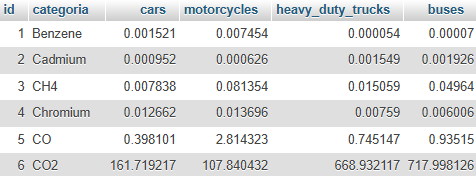
\includegraphics[width=0.75\linewidth]{foto/emission_factor.png}
    \vspace{0.3cm}
    \caption{Estratto della tabella dei Fattori di Emissione (ISPRA).}
    \label{fig:factors}
\end{figure}


\section{Il Modello di Stima delle Emissioni}

La piattaforma utilizza un modello volutamente semplice ma efficace, basato
sull'approccio \emph{attività $\times$ fattore di emissione}. L'idea è
trasformare un conteggio veicolare in una massa di inquinante emessa su un
certo tratto di strada.

\subsection{Formula di Calcolo Principale}

La massa totale di un inquinante $E_{\text{pollutant}}$ emessa su un tratto
stradale sorvegliato è calcolata come:

\begin{equation}
  E_{\text{pollutant}} =
    \sum_{\text{veicolo}} \left(
      \text{Conteggio}_{\text{veicolo}} \times
      \text{Lunghezza Tratto}_{\text{km}} \times
      \text{EF}_{\text{veicolo},\text{pollutant}}
    \right)
  \label{eq:emission_model}
\end{equation}
dove:
\begin{itemize}
  \item $\text{Conteggio}_{\text{veicolo}}$ è il conteggio totale dei veicoli
        di una certa categoria (es. auto, moto, bus, camion) nell'intervallo
        di tempo considerato;
  \item $\text{EF}_{\text{veicolo},\text{pollutant}}$ è il Fattore di
        Emissione (in $g/\text{veicolo}\cdot\text{km}$) per quella categoria
        di veicolo e per l'inquinante considerato;
  \item $\text{Lunghezza Tratto}_{\text{km}}$ è la lunghezza del tratto
        stradale (espressa in km) su cui si ritiene che il conteggio sia
        rappresentativo.
\end{itemize}

\subsection{Il Parametro di Lunghezza del Tratto (\texttt{path\_m})}

Poiché i dati di traffico vengono rilevati in un singolo punto
(la posizione della telecamera), è necessario introdurre un parametro che
descriva il tratto di strada a cui quel conteggio è effettivamente
riferito. In questa tesi tale informazione è rappresentata dal campo
\texttt{path\_m}, associato a ciascuna telecamera. Il parametro \texttt{path\_m} indica la lunghezza, espressa in metri,
del tratto di strada che si considera rappresentato da una determinata
telecamera. Si tratta di una proprietà geometrica del punto di
monitoraggio: può descrivere, ad esempio, un tratto di avvicinamento a
un incrocio, una porzione di viale urbano o un breve segmento di strada
a senso unico.

Nel modello di stima delle emissioni, la lunghezza utilizzata nella
Formula~\ref{eq:emission_model} è ottenuta convertendo il valore
memorizzato nel database in chilometri:

\[
  \text{Lunghezza Tratto}_{km} = \frac{\texttt{path\_m}}{1000}.
\]

In questo modo ogni telecamera contribuisce al calcolo con una lunghezza
specifica, scelta in base alle caratteristiche del sito di
monitoraggio. Il parametro \texttt{path\_m} viene impostato quando la
telecamera viene registrata nel sistema e rimane associato a quella
postazione per tutte le successive elaborazioni dei dati di traffico.

\section{Rappresentazione Geospaziale dei Dati}

\subsection{Librerie GIS e Punti di Interesse}

La libreria \textbf{Leaflet} viene utilizzata per rappresentare sulla mappa,
in modo interattivo, i punti di monitoraggio (telecamere) e i relativi valori
di traffico ed emissione. Ogni telecamera è memorizzata nel database con le
relative coordinate geografiche e con alcune informazioni descrittive (strada,
città, paese).

\subsection{Heatmap Dinamica tramite Circle Marker}

La scelta grafica adottata è una \textbf{heatmap discreta}, realizzata tramite
\texttt{L.circleMarker}. L'idea è quella di rappresentare ogni telecamera con
un cerchio il cui raggio e il cui colore dipendono dall'intensità del fenomeno
(conteggio o emissione).

Un modulo ausiliario svolge due compiti principali:
\begin{enumerate}
  \item \textbf{Normalizzazione:} il valore della
        metrica $v$ viene convertito in un numero $t$ compreso tra 0 e 1 in
        base al minimo e al massimo valori osservati nel dataset:
        \[
          t = \frac{v - \text{min}}{\text{max} - \text{min}}.
        \]
  \item \textbf{Stilizzazione dinamica:} il valore
        normalizzato $t$ viene mappato a un colore (scala dal verde al
        rosso) e a un raggio del marker. In questo modo la mappa mette subito
        in evidenza i punti più critici.
\end{enumerate}
Questa modalità di visualizzazione risulta intuitiva anche per chi non ha
una formazione specifica in modellistica ambientale, perché permette di
individuare rapidamente le zone con maggior traffico o maggior emissione
stimata.
% ======================================================================
% CAPITOLO 4 - ARCHITETTURA DEL SISTEMA
% ======================================================================

\chapter{Architettura del Sistema e Stack Tecnologico}
\section{Architettura Generale e Stack Tecnologico}

Il sistema segue una classica \textbf{architettura a tre livelli}
(\emph{Three-Tier Architecture}). Il primo livello è quello dei dati
(\emph{Database Server}), implementato con \textbf{MySQL}/MariaDB, che
contiene le tabelle con i conteggi di traffico, i metadati dei sensori e
i Fattori di Emissione. Il secondo livello è quello di applicazione
(\emph{Backend}), sviluppato in \textbf{PHP}, che riceve i file di
input, li trasforma in dati strutturati e risponde alle richieste del
frontend tramite API REST (come ad esempio \texttt{cameras.php}). Il
terzo livello è quello di presentazione (\emph{Frontend}), realizzato
in \textbf{HTML5}, \textbf{CSS3} e \textbf{JavaScript} (moduli ES6), in
cui risiedono la mappa Leaflet, i controlli grafici e il calcolo locale
delle emissioni. Le operazioni più pesanti in termini di I/O, come l'acquisizione di file
di log di grandi dimensioni, sono demandate al backend e al database.
Sul client rimangono invece i calcoli più leggeri ma ripetuti di
frequente, ad esempio il ricalcolo in tempo reale dell'inquinante o del
tipo di veicolo visualizzato sulla mappa.

\begin{figure}[H]
\caption{Schema compatto del flusso Backend: dai file grezzi alla visualizzazione in mappa.}
\centering
\begin{tikzpicture}[
  node distance=0.9cm,
  block/.style={
    rectangle,
    rounded corners=3pt,
    draw=black,
    thick,
    text width=5cm,
    text centered,
    minimum height=1.2cm,
    font=\scriptsize,
    align=center
  },
  flow/.style={->, thick, >=latex}
]

% --- FILE GREZZI --------------------------------------------------
\node[block, fill=gray!15] (raw) {
  \textbf{File dati grezzi}\\
  (CSV / TXT)
};

% --- upload_csv.php ------------------------------------------------
\node[block, fill=blue!15, below=of raw] (upload) {
  \texttt{upload\_csv.php}\\
  \small punto di ingresso dei file grezzi:\\
  prepara i dati e li scrive nel database
};

% --- DATABASE ------------------------------------------------------
\node[block, fill=green!15, below=of upload] (db) {
  Tabelle Database (intervalli aggregati)\\
  \texttt{traffic\_interval}\\
  \small 1 record per \texttt{camera\_id} e intervallo temporale
};

% --- API DI INTERROGAZIONE ----------------------------------------
\node[block, fill=orange!20, below left=1.2cm and -1.2cm of db] (api) {
  API di interrogazione\\
  \texttt{cameras.php}\\
  \small espone i dati aggregati verso il frontend
};

% --- FRONTEND ------------------------------------------------------
\node[block, fill=purple!15, below right=1.2cm and -1.2cm of db] (front) {
  Frontend\\
  \texttt{saved\_view.js}\\
  \small visualizza i dati sulla mappa (marker / heatmap)
};

% --- FRECCE --------------------------------------------------------
\draw[flow] (raw) -- (upload);
\draw[flow] (upload) -- (db);
\draw[flow] (db) -- (api);
\draw[flow] (api) -- (front);

\end{tikzpicture}
\end{figure}

\section{Modello Dati e Gestione dei Fattori di Emissione}

Il database, indicato di seguito come \texttt{traffico}, è strutturato
per rappresentare tre entità principali: la telecamera o il sensore, i
dati aggregati di traffico, che rappresentano intervalli temporali variabili con il conteggio dei vari veicoli e i coefficienti dei Fattori di Emissione.

\newpage
\subsection{Tabelle Principali del Database}

\begin{table}[h]
  \centering
  \caption{Schema del modello dati semplificato}
  \label{tab:schema_dati}
  \begin{tabularx}{\linewidth}{|l|X|X|}
    \hline
    \textbf{Tabella} & \textbf{Contenuto} & \textbf{Campi principali} \\
    \hline
        \texttt{camera}
      & Metadati dei sensori/telecamere
      & \texttt{camera\_id} (PK), \texttt{lat}, \texttt{lon}, \texttt{road},
        \texttt{city}, \texttt{province}, \texttt{region},
        \texttt{country\_iso2}, \texttt{path\_m} \\
    \hline
    \texttt{traffic\_interval}
      & Conteggi veicolari aggregati per intervallo
      & \texttt{camera\_id} (FK), \texttt{ts\_start}, \texttt{interval\_s},
        \texttt{cars}, \texttt{motos}, \texttt{buses}, \texttt{trucks} \\
    \hline
    \texttt{emissioni\_gkm}
      & Fattori di Emissione per inquinante
      & \texttt{categoria}, \texttt{cars}, \texttt{motorcycles},
        \texttt{heavy\_duty\_trucks}, \texttt{buses} \\
    \hline
  \end{tabularx}
\end{table}

\subsection{Gestione dei Fattori di Emissione (\texttt{EF})}

La tabella \texttt{emissioni\_gkm} contiene i coefficienti EF utilizzati
dal modello dell’Equazione~\ref{eq:emission_model}. Per migliorare le
prestazioni, questi fattori vengono caricati in un’unica soluzione dal
backend tramite una specifica API e memorizzati sul
client in una struttura dati dedicata. In
termini di flusso dei dati, il backend espone i valori grezzi dei
Fattori di Emissione, mentre il frontend li utilizza per trasformare i
conteggi di traffico in emissioni stimate senza dover effettuare nuove
chiamate al server ogni volta che l’utente cambia inquinante o categoria
veicolare.

\section{Interfacce di Comunicazione (API)}

Per collegare il livello di acquisizione dei dati con quello di visualizzazione,
il sistema utilizza alcune API che definiscono in modo chiaro quali informazioni
devono essere scambiate tra backend e frontend. Queste interfacce regolano il
flusso dei dati lungo l’intero percorso: dall’arrivo dei file grezzi fino alla loro
interpretazione sulla mappa. Di seguito se ne descrivono le funzioni principali,
senza entrare nei dettagli implementativi approfonditi (affrontati nel
Capitolo~\ref{ch:backend}).

\subsection{API di Acquisizione Dati (\texttt{upload\_csv.php})}

L’API \texttt{upload\_csv.php} rappresenta il punto di ingresso dei file
di conteggio provenienti dal sistema di rilevamento video. Il servizio legge i
file \texttt{TXT}/\texttt{CSV}, interpreta i metadati associati e organizza le
rilevazioni in intervalli temporali regolari da inserire nella tabella
\texttt{traffic\_interval}. Quando il file proviene da una telecamera non ancora registrata, l’API richiede
anche il valore \texttt{path\_m}, ovvero la lunghezza del tratto stradale associato a
quella postazione. Questo parametro viene salvato nella tabella \texttt{camera} e
mantiene un valore stabile nel tempo, così da garantire coerenza nei caricamenti
successivi. Se \texttt{path\_m} manca o non è valido, l’API interrompe
l’importazione e restituisce un messaggio di errore chiaro all’utente.

\subsection{API di Query Dati (\texttt{cameras.php})}

L’API \texttt{cameras.php} fornisce al frontend i dati aggregati necessari alla
visualizzazione sulla mappa. Riceve come input i parametri scelti dall’utente
(intervallo temporale, area geografica ed eventuali opzioni di dettaglio),
seleziona le telecamere pertinenti e costruisce una risposta JSON che include:

\begin{itemize}
  \item informazioni geografiche della telecamera;
  \item conteggi aggregati dei veicoli;
  \item statistiche utili alla normalizzazione dei valori (min/max);
  \item eventuali serie temporali dettagliate per il Player Giornaliero.
\end{itemize}

In pratica, \texttt{cameras.php} è l’anello di congiunzione tra i dati conservati
nel database e la rappresentazione interattiva offerta dal frontend.

\subsection{API Fattori di Emissione (\texttt{emission\_factor.php})}

L’API \texttt{emission\_factor.php} espone al frontend i Fattori di
Emissione memorizzati nella tabella \texttt{emissioni\_gkm}. Questa chiamata
avviene tipicamente una sola volta all’avvio dell’applicazione, così da caricare
tutti i coefficienti necessari al calcolo delle emissioni per categoria veicolare.
Una volta trasferiti al client, tali valori possono essere riutilizzati localmente
senza dover richiedere ulteriori operazioni al server, migliorando fluidità e tempi
di risposta.

% ======================================================================
% CAPITOLO 5 - BACKEND
% ======================================================================
\chapter{Implementazione del Backend: Dati e Calcolo}
\label{ch:backend}

Come anticipato nel Capitolo~4, il backend ha il compito di trasformare
file di conteggio grezzi in serie temporali aggregate e di renderle
disponibili al frontend tramite API. In questo capitolo si entra nel
dettaglio del \emph{comportamento} dei servizi lato server, descrivendo
le scelte implementative adottate e le principali logiche di controllo
ed aggregazione.

\section{Processo di Acquisizione e Pre-elaborazione Dati}

L’acquisizione dei dati grezzi, tipicamente in formato CSV/TXT, è
gestita da un’apposita API del backend, implementata nel servizio
\texttt{upload\_csv.php}. Questo componente rappresenta il punto di
ingresso del sistema: riceve i file generati dal processo di
rilevamento (YOLO + tracking) e li trasforma in dati strutturati. Il servizio non si limita a salvare il contenuto nel database, ma
applica una serie di controlli fondamentali per garantirne la qualità:
verifica la coerenza del file, associa correttamente il flusso dati alla
telecamera di riferimento, aggrega gli eventi in 
\begin{wrapfigure}{l}{0.40\textwidth}
    \vspace{-8pt}
    \centering
    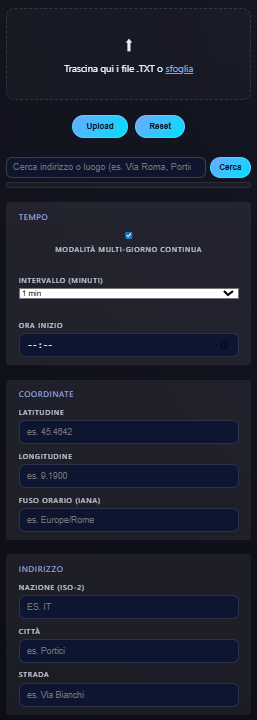
\includegraphics[width=\linewidth]{foto/Screenshot 2025-11-24 152305.png}
    \caption{Menù salvataggio}
    \vspace{-8pt}
\end{wrapfigure}

intervalli temporali
regolari (\emph{time bucketing}) ed evita la sovrapposizione con dati
già presenti. Una volta lette le rilevazioni grezze, il sistema deve trasformare la
sequenza di detection frame-by-frame in un insieme di valori realmente
utilizzabili. Ogni riga del file rappresenta infatti la presenza di un
veicolo in un certo frame, ma non corrisponde necessariamente a un
passaggio. Per ottenere un conteggio significativo, il backend suddivide
l’asse temporale in intervalli regolari (un minimo di 1 minuto per un massimo di un ora)
e accumula tutte le rilevazioni che rientrano nello stesso intervallo.
Ogni intervallo produce quindi un unico record che riassume quanti
veicoli sono stati osservati e a quali categorie appartengono (auto,
moto, bus, camion). Questo processo riduce il rumore, rende i dati
omogenei tra telecamere diverse e permette al frontend di lavorare su
una serie temporale compatta e coerente.

La logica complessiva dell’acquisizione si articola in tre fasi
principali:

\begin{itemize}
  \item \textbf{Definizione Logica del Sensore:} i metadati contenuti nel file
  (posizione, strada, città e, per le nuove telecamere, la lunghezza del
  tratto \texttt{path\_m}) vengono utilizzati per identificare la
  telecamera corrispondente. Se non è presente nel database, il sistema
  ne crea automaticamente una nuova, registrando anche il valore
  \texttt{path\_m} nella tabella \texttt{camera}.


  \item \textbf{Aggregazione dei passaggi:} le rilevazioni vengono
  raggruppate in intervalli temporali della durata scelta al momento del
  caricamento e inserite nella tabella \texttt{traffic\_interval}.

  \item \textbf{Gestione delle anomalie:} il servizio rileva eventuali
  sovrapposizioni temporali o duplicati; in questi casi segnala il
  problema all’interfaccia ed esclude soltanto i record in conflitto.
\end{itemize}

Al termine dell’elaborazione, l’API \texttt{upload\_csv.php} restituisce
un risultato in formato JSON che riporta il numero di intervalli
correttamente inseriti, quelli ignorati e gli eventuali avvisi.

\begin{figure}[H]
    \centering
    \vspace{0.3cm}
    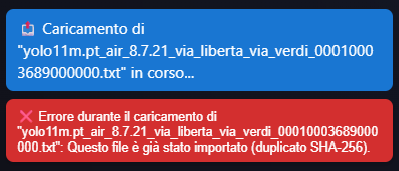
\includegraphics[width=0.75\linewidth]{foto/error_duplicato.png}
    \caption{Esempi messaggi e errori}
    \vspace{0.0cm}
\end{figure}

\begin{figure}[H]
    \centering
    \vspace{0.0cm}
    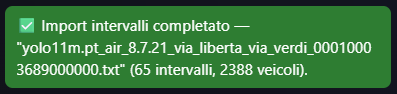
\includegraphics[width=0.75\linewidth]{foto/inport_riuscito.png}
    \vspace{0.3cm}
\end{figure}

\section{Logica di Aggregazione e Interrogazione}

Per la visualizzazione sulla mappa e per le analisi successive, il
backend mette a disposizione un servizio di interrogazione,
implementato nell’API \texttt{cameras.php}, che funge da \emph{data
provider} per il frontend. Questa API riceve come input l’intervallo
temporale richiesto, il luogo da analizzare e alcune opzioni aggiuntive.
A partire da tali parametri, il servizio costruisce dinamicamente la
query verso la tabella \texttt{traffic\_interval} e restituisce per ogni
telecamera un insieme di dati già aggregato e pronto per la
rappresentazione.

La logica interna è organizzata in più passaggi:

\begin{itemize}
  \item \textbf{Selezione delle telecamere:} sulla base del luogo
  indicato (città, provincia o Paese), il sistema individua le
  telecamere rilevanti.

  \item \textbf{Filtraggio temporale:} vengono estratti solo gli
  intervalli che ricadono nella finestra di tempo richiesta.

  \item \textbf{Aggregazione per telecamera:} per ciascun sensore
  vengono calcolate le somme dei passaggi per categoria veicolare e il
  totale complessivo.

  \item \textbf{Calcolo delle statistiche globali:} l’API determina i
  valori minimi e massimi necessari al frontend per normalizzare i dati
  nella heatmap.

  \item \textbf{Costruzione della risposta:} il servizio produce un
  oggetto JSON contenente, per ogni telecamera, coordinate, descrizione,
  conteggi aggregati, statistiche globali ed eventuali serie temporali
  dettagliate.
\end{itemize}

Nel caso di parametri mancanti o non validi, l’API \texttt{cameras.php}
genera una risposta strutturata con codici e messaggi di errore,
permettendo al frontend di informare correttamente l’utente.


% ======================================================================
% CAPITOLO 6 - FRONTEND
% ======================================================================

\chapter{Implementazione del Frontend: Visualizzazione Interattiva}Questo capitolo descrive il funzionamento del frontend, con particolare attenzione alla logica di calcolo lato client, alla visualizzazione georeferenziata sulla mappa e all'interazione con l'utente.

\section{Il Modulo delle Metriche e il Calcolo}La logica di calcolo lato client è centralizzata in un modulo specifico, che rappresenta il “cuore” della trasformazione dei dati aggregati in valori di emissione. Questo modulo è responsabile della gestione dello stato della metrica, dell'applicazione della formula di stima e del caricamento dei Fattori di Emissione.

\subsection{Gestione dello Stato e Inizializzazione dei Fattori di Emissione}

Il modulo delle metriche gestisce due aspetti centrali che determinano ciò che
viene visualizzato sulla mappa: la categoria veicolare selezionata (ad esempio
totale, veicoli pesanti, autovetture) e la metrica di analisi, che stabilisce se la
visualizzazione deve basarsi sul conteggio grezzo oppure su un inquinante
specifico (es. NOX, PM\textsubscript{10}).

\begin{wrapfigure}{l}{0.40\textwidth}
    \vspace{-8pt}
    \centering
    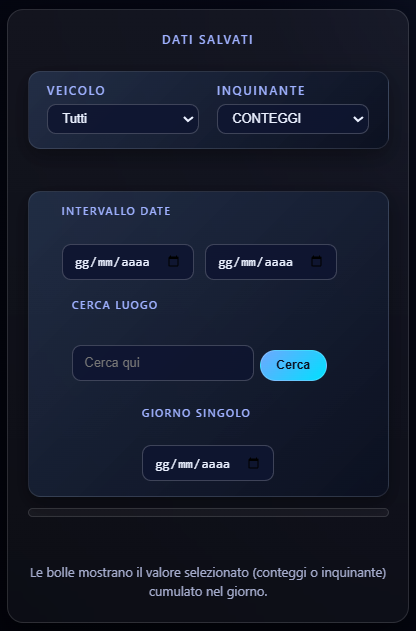
\includegraphics[width=\linewidth]{foto/menu_salvati.png}
    \caption{Menù salvati}
    \vspace{-8pt}
\end{wrapfigure}

Le scelte dell’utente vengono mantenute dal modulo e trasmesse agli altri
componenti dell’interfaccia, che aggiornano automaticamente la mappa.
Quando l’utente modifica il tipo di veicolo o l’inquinante, il sistema ricalcola
immediatamente i valori per tutte le telecamere, garantendo una risposta fluida
e coerente.

Prima del calcolo delle emissioni, il modulo inizializza la struttura dati dei
Fattori di Emissione richiedendoli all’API dedicata. Questi valori vengono
caricati una sola volta all’avvio e riutilizzati per tutte le operazioni successive,
evitando chiamate ridondanti al backend.

\subsection{Formulazione e Selezione della Metrica (Conteggio vs Emissione)}

La funzione principale del modulo riceve in input i conteggi aggregati relativi a
ciascuna telecamera e restituisce un valore numerico normalizzato da utilizzare
per la rappresentazione in mappa. Il processo è selettivo:

\begin{enumerate}
\item se la metrica corrente è il conteggio, viene restituito il totale dei veicoli
oppure il valore relativo alla categoria selezionata;
\item se la metrica è un inquinante, viene applicata la relazione definita
nell'Equazione~\ref{eq:emission_model}, combinando conteggi aggregati,
Fattori di Emissione e lunghezza del tratto associata alla telecamera
(\texttt{path\_m}). Tale valore, convertito in chilometri, permette di rapportare
l’attività veicolare al tratto stradale rappresentato dal sensore.
\end{enumerate}

\section{Mappa e Rappresentazione Heatmap}

La visualizzazione geografica è affidata a un modulo dedicato che sfrutta la
libreria \textbf{Leaflet} per inizializzare la mappa, gestire i layer e posizionare i
marker corrispondenti alle telecamere.

\begin{figure}[H]
    \centering
    \vspace{0.3cm}
    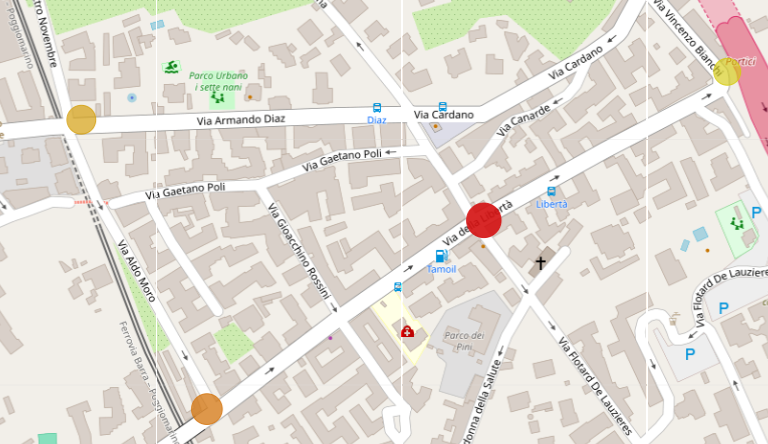
\includegraphics[width=0.75\linewidth]{foto/circle_marker.png}
    \caption{Heatmap portici}
    \vspace{0.3cm}
\end{figure}

\subsection{Visualizzazione Geospaziale tramite Leaflet}

Ogni telecamera è rappresentata da un \emph{circle marker} con colore e raggio
proporzionali al valore normalizzato della metrica. Questa scelta consente di
realizzare una heatmap discreta che mette rapidamente in evidenza le aree più
significative. Quando l’utente modifica la metrica o il tipo di veicolo, i marker vengono
aggiornati immediatamente senza ricaricare la mappa. Leaflet gestisce inoltre
funzionalità come \emph{panning}, zoom e \emph{fitBounds}, utili per centrare la
vista sulle telecamere selezionate.

\subsection{Normalizzazione, Scala Colore e Circle Marker}

Un modulo ausiliario traduce i valori numerici calcolati dalla logica delle metriche
in elementi grafici coerenti. Le operazioni principali sono:

\begin{itemize}
\item \textbf{Normalizzazione:} conversione del valore assoluto (conteggio o
emissione) nell’intervallo $[0,1]$;
\item \textbf{Stilizzazione:} assegnazione di colore, raggio e opacità proporzionali;
\item \textbf{Visualizzazione:} creazione e aggiornamento dinamico dei
\texttt{CircleMarker} sulla mappa.
\end{itemize}

La scala cromatica dal verde (valori bassi) al rosso (valori alti) rappresenta una
convenzione visiva immediata e ampiamente utilizzata nel contesto ambientale.

\section{Interfaccia Utente e Controlli Interattivi}

Un componente dedicato collega i controlli dell'interfaccia (selettori di data,
luogo, metrica e pulsante di ricerca) con il backend e con la logica di
visualizzazione. Quando viene avviata una ricerca, il modulo raccoglie i parametri
selezionati, invia una richiesta all’API \texttt{cameras.php} e genera i marker
corrispondenti sulla mappa. I cambiamenti di metrica (ad esempio dal conteggio a un inquinante) non
richiedono nuove chiamate al server: l’aggiornamento avviene localmente,
ricalcolando solo i valori e lo stile dei marker già presenti.

\section{Componenti Accessori: Grafici e Player Giornaliero}

\subsection{Popups e Dettagli del Marker}

Un modulo genera il contenuto HTML dei popup associati ai marker.
Ogni popup mostra informazioni contestuali: descrizione del luogo, valore della
metrica corrente e dettaglio dei conteggi per categoria veicolare.

\begin{figure}[H]
    \centering
    \vspace{0.3cm}
    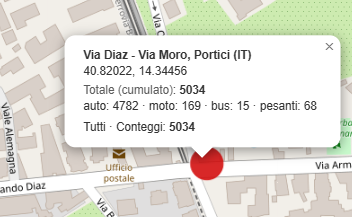
\includegraphics[width=0.75\linewidth]{foto/popUp.png}
    \caption{Popup informativo}
    \vspace{0.3cm}
\end{figure}

\begin{figure}[H]
    \centering
    \vspace{0.3cm}
    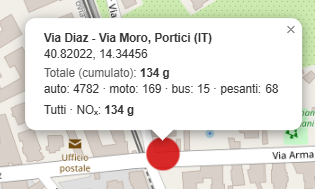
\includegraphics[width=0.75\linewidth]{foto/popUp1.png}
    \vspace{0.3cm}
\end{figure}


\subsection{Grafici e Analisi Aggiuntive}

Per un’analisi più sintetica, viene utilizzata la libreria Chart.js per produrre:

\begin{enumerate}
\item un \textbf{grafico a torta} che mostra la ripartizione delle emissioni tra gli
inquinanti considerati;
\item un \textbf{grafico orario medio}, che evidenzia l’andamento giornaliero del
traffico o delle emissioni.
\end{enumerate}

\begin{figure}[h!]
    \centering
    \begin{minipage}{0.48\linewidth}
        \centering
        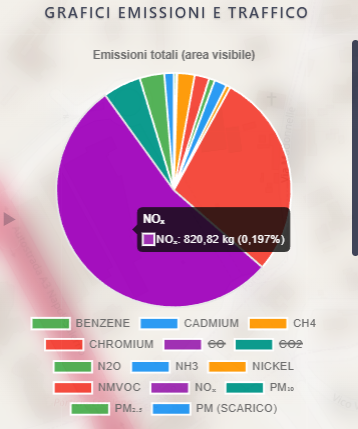
\includegraphics[width=\linewidth]{foto/Pies_saved.png}
        \caption{Grafico a torta inquinanti}
    \end{minipage}\hfill
    \begin{minipage}{0.48\linewidth}
        \centering
        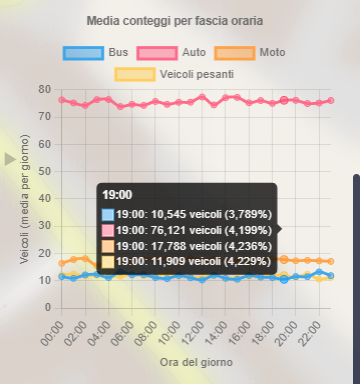
\includegraphics[width=\linewidth]{foto/graph_saved.png}
        \caption{Grafico media oraria veicoli}
    \end{minipage}
\end{figure}

I grafici utilizzano le etichette (\textit{labels}), i valori numerici (\textit{data})
e le opzioni di stile fornite al modulo, consentendo una rappresentazione
immediata dell’evoluzione temporale e della composizione delle emissioni.

\subsection{Player Giornaliero Dinamico}

Quando il backend fornisce serie temporali dettagliate, un componente permette
di far scorrere gli intervalli temporali come i frame di un’animazione. Ad ogni
passo la mappa viene aggiornata, mostrando l’evoluzione del traffico e delle
emissioni durante l’arco della giornata.

\begin{figure}[H]
    \centering
    \vspace{0.3cm}
    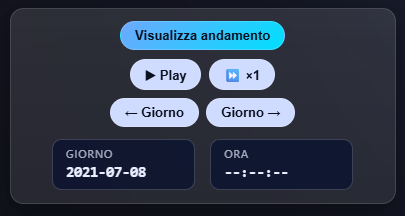
\includegraphics[width=0.9\linewidth]{foto/player.png}
    \vspace{0.3cm}
\end{figure}

% ======================================================================
% CAPITOLO 7 - RISULTATI E SVILUPPI FUTURI
% ======================================================================

\chapter{Risultati e Valutazioni}

In questo capitolo vengono riassunti i risultati ottenuti, discusse le principali
implicazioni del modello di calcolo e dell'approccio adottato, e proposte
alcune possibili direzioni di sviluppo futuro.



\section{Risultati Operativi del Modello di Stima}

Dal punto di vista operativo, la piattaforma ha dimostrato di essere efficace in diverse funzionalità chiave: utilizza in tempo reale la formula di stima delle emissioni a partire dai conteggi veicolari aggregati, combina i dati di traffico con Fattori di Emissione ufficiali forniti da enti come ISPRA e consente il passaggio rapido tra una visualizzazione basata sul semplice conteggio dei veicoli e una visualizzazione basata sulle emissioni stimate.

Nel complesso, il modello risulta particolarmente adatto a rappresentazioni
comparative tra diverse zone della città o tra diversi periodi temporali. La sua utilità è quindi maggiore nell'analisi relativa che nella stima puntuale e assoluta della concentrazione di inquinanti in un punto specifico.

\subsection{Implicazioni del Parametro \texttt{path\_m}}

Il parametro \texttt{path\_m} svolge un ruolo centrale nel collegare i
conteggi veicolari alle stime di emissione. Attribuire a ciascuna
telecamera una lunghezza specifica consente di interpretare i dati non
solo come numero di veicoli transitati in un punto, ma come attività
veicolare riferita a un tratto di strada di ampiezza nota.

Una lunghezza maggiore indica un tratto più esteso rappresentato dal sensore e, a parità di conteggio, comporta un livello di attività e di emissione proporzionalmente più elevato. Questo permette di distinguere in modo naturale tra postazioni collocate in incroci molto compatti e punti situati lungo assi viari più ampi o continui.
L’adozione di \texttt{path\_m} introduce tuttavia alcune assunzioni. Si
presume che il tratto associato alla telecamera sia rappresentativo, in media, della porzione di strada effettivamente influenzata dal sensore e che tale valore rimanga stabile nel tempo. Inoltre, la lunghezza è considerata come proprietà complessiva del sito di monitoraggio, senza distinguere tra corsie o direzioni di marcia. Per questi motivi, i risultati ottenuti sono particolarmente adatti a confronti relativi tra punti o periodi diversi, più che a stime puntuali da utilizzare in modo diretto in contesti normativi.

\section{Efficacia della Visualizzazione Heatmap}

L'uso della mappa con cerchi colorati (intesa come heatmap discreta) si è rivelato intuitivo e facilmente leggibile. La possibilità di cambiare in modo interattivo il tipo di veicolo o di inquinante da visualizzare rende la piattaforma flessibile e adatta a diversi scenari d'uso, dall'analisi accademica ai contesti più applicativi (come la pianificazione di Zone a Traffico Limitato o l'analisi degli orari di punta).

\subsection{Robustezza del Processo di Acquisizione}

Il meccanismo di auto-accodamento dei dati e l'uso delle transazioni per il salvataggio hanno reso il processo di acquisizione dati sufficientemente robusto anche in presenza di file parziali o con sovrapposizioni temporali. Questo aspetto è di grande importanza, in quanto la raccolta dei dati sul campo avviene spesso in più sessioni, con possibili disallineamenti temporali.

\chapter{Conclusioni e Prospettive Future}

\section{Conclusioni}

In conclusione, il progetto ha raggiunto l'obiettivo principale prefissato: la realizzazione di una piattaforma web completa che consenta di:
\begin{itemize}
 \item caricare, gestire e pre-elaborare dati di traffico provenienti da telecamere o sensori;
 \item stimare, con un modello semplice ma coerente, le emissioni di alcuni inquinanti atmosferici;
 \item visualizzare i risultati di questi calcoli in maniera interattiva e georeferenziata.
\end{itemize}

La chiara separazione tra il backend (gestione e aggregazione dati) e il frontend (calcolo delle emissioni e visualizzazione) ha contribuito a mantenere il sistema flessibile, manutenibile e relativamente semplice da estendere per futuri sviluppi.

\section{Prospettive per Sviluppi Futuri}

Tra gli sviluppi futuri possibili, si segnalano le seguenti direzioni:
\begin{itemize}
 \item l'implementazione di modelli di emissione più avanzati, in grado di tenere conto di fattori variabili come le fasi di avviamento a freddo, la velocità media o la pendenza del tratto stradale rilevato;
 \item l'aggiunta di modelli per un riconoscimento più specifico del tipo di veicolo, in grado di distinguere tra mezzi elettrici, benzina o diesel.
\end{itemize}

Questi sviluppi permetterebbero di trasformare la piattaforma da strumento di analisi prevalentemente descrittiva a strumento di supporto più avanzato per la pianificazione e la gestione strategica della mobilità urbana.

% ======================================================================
% APPENDICI
% ======================================================================
\newpage
\thispagestyle{empty}
\mbox{}
\newpage

\chapter*{Ringraziamenti}

Giungere a questo traguardo non sarebbe stato possibile senza il sostegno, l'amore e la pazienza di molte persone straordinarie che desidero ringraziare di cuore.

\section*{La Mia Famiglia}

Rivolgo il mio primo e più sentito ringraziamento ai miei genitori, a mia Madre e a mio Padre. Siete stati il mio faro e il mio rifugio in ogni momento: avete creduto in me quando nemmeno io ci riuscivo, avete affrontato sacrifici silenziosi e continui, e mi avete donato un amore che ha reso ogni ostacolo più leggero.
Grazie per avermi insegnato cosa significa impegnarsi davvero, per non avermi mai lasciato indietro, e per avermi sostenuto in ogni scelta.
\vspace{0.5cm}

Un grazie speciale va anche a te, mia sorella. Sei sempre presente, con una pazienza e un aiuto costante. La tua vicinanza ha reso più lieve ogni momento difficile, e sapere di poter contare su di te ha reso questo cammino molto più bello.

\vspace{0.5cm}

Un ringraziamento speciale va ai miei zii. Grazie per l’affetto sincero, per gli incoraggiamenti che non sono mai mancati e per la vostra presenza rassicurante. Siete stati un punto di riferimento stabile, pronti a sostenere, a sorridere e a offrire una parola giusta quando serviva davvero.
\newpage


Un ringraziamento altrettanto sentito va a voi, miei cugini. Con voi ho condiviso leggerezza, complicità e tanti momenti che hanno alleggerito questo percorso. La vostra gioia spontanea e la vostra vicinanza hanno reso tutto più sereno, anche perchè voi c'eravate già passati.
\vspace{0.5cm}

Il mio pensiero più profondo va ai miei nonni  a chi è ancora qui con me e a chi, purtroppo, non può essere presente. Vi sento vicini in ogni mio successo. Il vostro esempio, il vostro amore e i vostri insegnamenti sono stati per me un’ispirazione costante e un vero e proprio punto di riferimento.
Sono certo che oggi starete gioendo con me, e questo pensiero mi accompagna con forza e gratitudine.

\section*{Gli Amici}

Ringrazio di cuore tutti i miei Amici, i compagni di avventura di una vita. Siete stati la mia valvola di sfogo, la fonte di risate e di spensieratezza necessarie per affrontare lo studio con la giusta leggerezza. Grazie per aver condiviso con me le fatiche e, soprattutto, le immense gioie di questo percorso.

Un ringraziamento speciale è riservato alla "Crème", il nucleo di persone incredibili che ha saputo starmi accanto con un supporto emotivo e pratico insostituibile. A voi, grazie per i consigli sinceri, per le notti passate tra Gianni e Garage, e per essere la mia vera e propria famiglia scelta. Siete l'eccellenza, e non potrei desiderare compagnia migliore.


\section*{I Miei Colleghi}

Rivolgo un ringraziamento di cuore ai compagni di corso, i veri compagni di questa lunga e estenuante avventura accademica.
Un grazie speciale a coloro che hanno saputo condividere appunti, studio e soprattutto caffè con encomiabile spirito di squadra.
Senza le vostre gag e il vostro supporto reciproco, probabilmente starei ancora cercando di capire la prima slide. Siete stati la mia guida. 


\vspace{1cm}
Grazie a tutti per aver reso questo percorso meno solitario e infinitamente più bello.
Abbiamo vinto!
\end{document}
